\documentclass[border=10pt]{standalone}
\usepackage[svgnames]{xcolor}
\usepackage{amsmath}
\usepackage{pgfplots}
\pgfplotsset{compat=newest}
\usepackage[sfdefault]{FiraSans}
\usepackage{FiraMono}
\renewcommand*\familydefault{\sfdefault}
\begin{document}
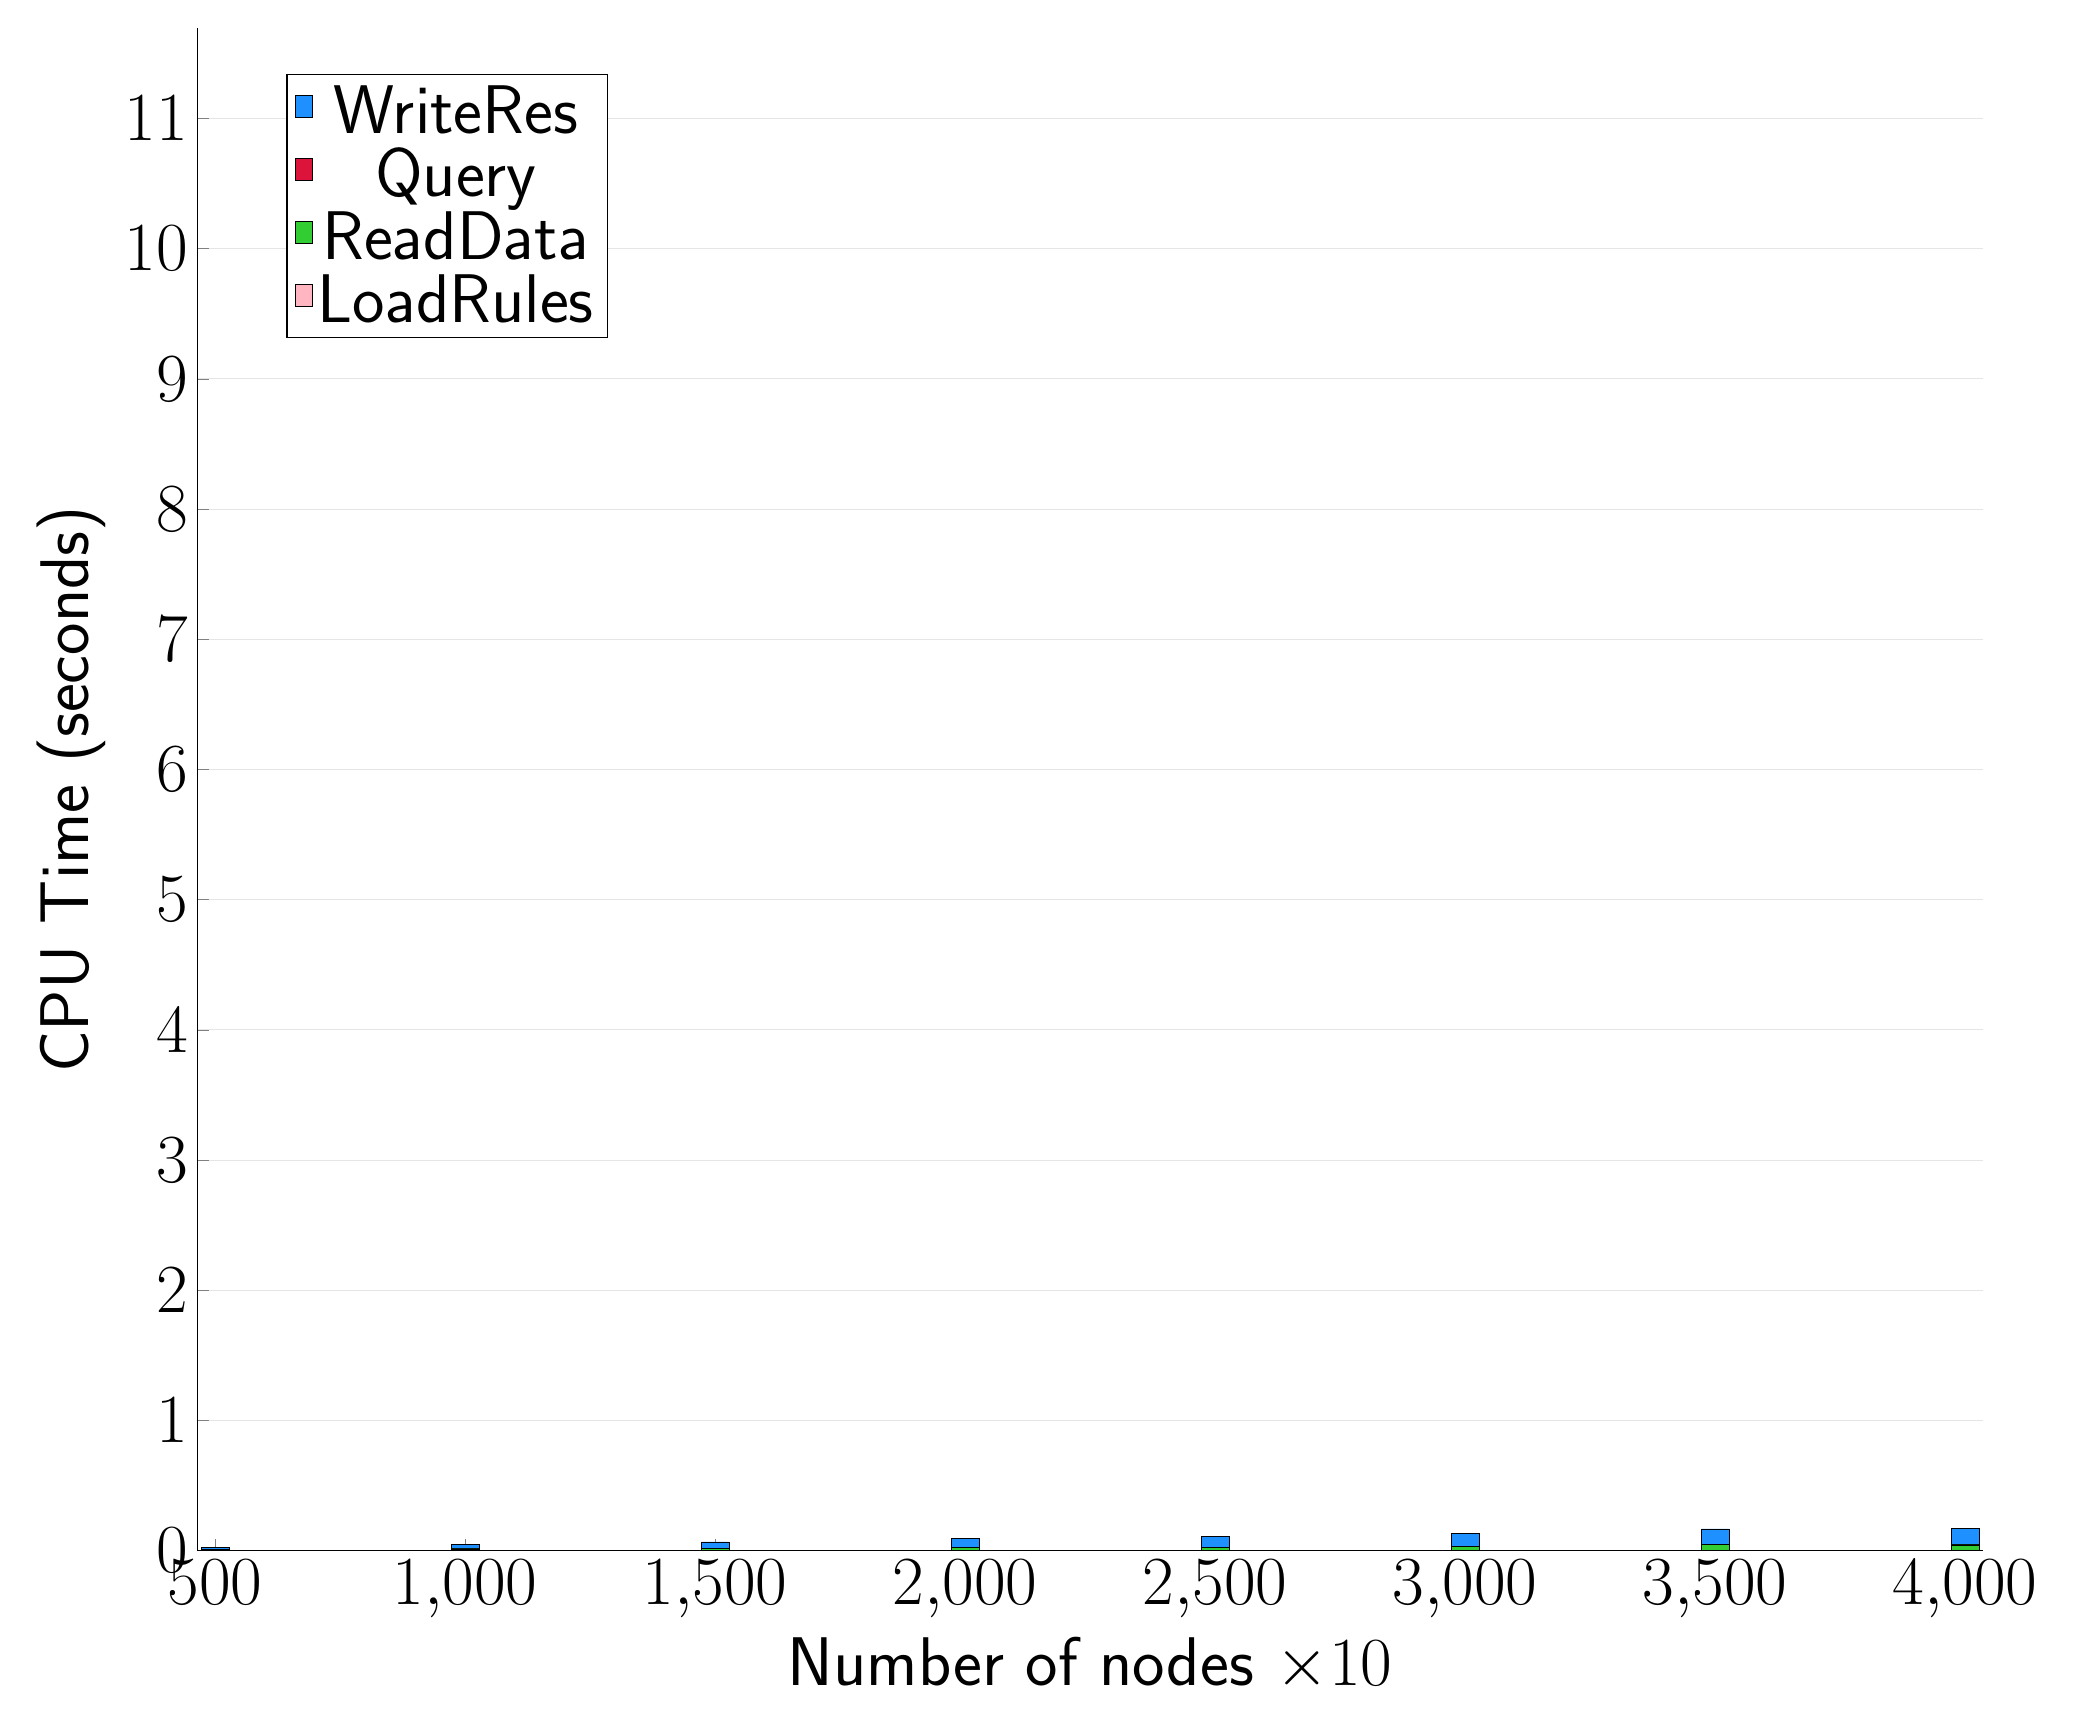
\begin{tikzpicture}
\begin{axis}[
   ybar stacked,
   width=2\textwidth,
   bar width=0.35cm,
   ymajorgrids, tick align=inside,
   major grid style={draw=gray!20},
   xtick=data,
   ymin=0, ymax=11.693333332737287,
   axis x line*=bottom,
   axis y line*=left,
   enlarge x limits=0.01,
   legend style={
       at={(0.23, 0.97)},
       anchor=north east,
       legend columns=1,
       font=\Huge,
   },
   ylabel={CPU Time (seconds)},
   xlabel={Number of nodes $\times 10$},
   label style={font=\Huge},
   tick label style={font=\Huge},
]
\addlegendimage{fill=DodgerBlue, draw=black, line width=0.2pt}
\addlegendentry{WriteRes}
\addlegendimage{fill=Crimson, draw=black, line width=0.2pt}
\addlegendentry{Query}
\addlegendimage{fill=LimeGreen, draw=black, line width=0.2pt}
\addlegendentry{ReadData}
\addlegendimage{fill=LightPink, draw=black, line width=0.2pt}
\addlegendentry{LoadRules}
\addplot +[fill=LightPink, draw=black, line width=0.2pt] coordinates {
(500, 0.0035803333333333334)
(1000, 0.003021)
(1500, 0.0029533333333333334)
(2000, 0.0036346666666666667)
(2500, 0.002138666666666668)
(3000, 0.003101)
(3500, 0.0037143333333333334)
(4000, 0.002484)
};
\addplot +[fill=LimeGreen, draw=black, line width=0.2pt] coordinates {
(500, 0.006072000000000001)
(1000, 0.011245666666666666)
(1500, 0.016856)
(2000, 0.023018333333333335)
(2500, 0.024979333333333336)
(3000, 0.030097333333333337)
(3500, 0.042278333333333334)
(4000, 0.04171666666666667)
};
\addplot +[fill=Crimson, draw=black, line width=0.2pt] coordinates {
(500, 0.00018533333333333566)
(1000, 0.00025399999999999734)
(1500, 0.0003856666666666683)
(2000, 0.0006050000000000013)
(2500, 0.000678999999999999)
(3000, 0.0008340000000000017)
(3500, 0.0013499999999999968)
(4000, 0.0013066666666666667)
};
\addplot +[fill=DodgerBlue, draw=black, line width=0.2pt] coordinates {
(500, 0.016182)
(1000, 0.032174666666666664)
(1500, 0.047274000000000004)
(2000, 0.06681533333333332)
(2500, 0.082085)
(3000, 0.099611)
(3500, 0.119356)
(4000, 0.1272033333333333)
};
\end{axis}
\end{tikzpicture}

\end{document}
